\chapter{Application Implementation and User Experience}
\label{chap:application-ux}

The preceding chapters describe the processing and retrieval mechanisms that make the assistant useful. This chapter focuses on how those mechanisms are assembled into an application that a user can operate and inspect. The implementation follows a modular-monolith structure: a browser client communicates with one ASP.NET Core application, which owns the domain services, persistence access, provider adapters, background processing, and delivery of the compiled client. This shape is appropriate for the present project because it keeps ownership rules and data consistency inside one deployable backend while still separating responsibilities in code.

The user interface is deliberately chat-first, but the chat is not the whole product. A workspace holds a reusable document collection and a persistent set of conversations. Separate document screens expose ingestion state and technical diagnostics, while source dialogs connect an answer back to stored provenance. These elements make the processing pipeline visible enough for debugging and evaluation without requiring an ordinary user to understand vectors, token counts, or ranking formulas.

\section{Technology Stack}
\label{sec:technology-stack}

Table~\ref{tab:technology-stack} summarizes the principal technologies and their roles. The table describes their use in this application rather than attempting a general comparison of web frameworks or databases. Version-specific claims in the final submission should be checked once more against the locked project files.

\begin{table}[!htbp]
    \centering
    \caption{Principal technologies and their roles in the application.}
    \label{tab:technology-stack}
    \small
    \begin{tabular}{L{0.23\textwidth} L{0.31\textwidth} L{0.36\textwidth}}
        \toprule
        \textbf{Technology} & \textbf{Role} & \textbf{Reason for use in this project} \\
        \midrule
        .NET and ASP.NET Core & JSON API, authentication host, dependency composition, background worker, and static client hosting & Provides one typed server environment for authorization, processing orchestration, and model-provider boundaries. \\
        Entity Framework Core & Relational mapping and database access & Expresses ownership and cascade relationships and keeps transactional persistence in the application data model. \\
        PostgreSQL & Durable relational storage and full-text retrieval & Stores users, workspaces, documents, processing artifacts, conversations, and generated search vectors in one database. \\
        pgvector & Native embedding column and cosine search & Keeps vectors beside their owning chunks and allows project-filtered similarity queries in PostgreSQL. \\
        React and TypeScript & Single-page browser interface & Supports reusable typed views for workspaces, chat, documents, dialogs, and asynchronous feedback. \\
        PdfPig & Native PDF text and structural inspection & Supplies page text, page geometry, and raster-image placement information without requiring page rendering. \\
        Open XML SDK & DOCX extraction & Reads paragraphs, heading styles, and table content from the document package in source order. \\
        PDFtoImage/PDFium & Local rendering of selected PDF pages & Produces bounded raster images only for pages routed to optical character recognition (OCR). \\
        Tesseract & Local OCR engine & Recognizes Romanian and English text from selected scan-like pages without using a cloud OCR service. \\
        OpenAI API and .NET SDK & Embeddings, structured document understanding, reranking, and grounded answer generation & Places each model-dependent operation behind a narrow adapter while the backend retains validation and authorization authority. \\
        \bottomrule
    \end{tabular}
\end{table}

The server targets .NET 10. The client uses React 19 and TypeScript and is built with Vite. PostgreSQL is not used merely as a conventional record store: the application also relies on a generated full-text search column with a Generalized Inverted Index (GIN) and a fixed-size \texttt{vector(1536)} column. This reduces the number of separate infrastructure components needed for a bachelor-project implementation. It also means that deleting a document through its relational ownership path removes its chunks and their vectors through the same database lifecycle.

External model access is restricted to explicit application services. The browser never receives provider credentials, physical upload paths, stored filenames, system instructions, or raw provider responses. The server supplies only the contracts needed by the current screen. Local extraction and OCR services likewise have narrow boundaries: a PDF renderer renders a requested page under a safety limit, while the OCR service recognizes the supplied image. This separation makes the implementation easier to substitute in tests and prevents UI concerns from acquiring file-system or provider responsibilities.

\section{Authentication and Workspaces}
\label{sec:authentication-workspaces}

The application uses the following user-facing hierarchy:

\begin{center}
\textbf{User} $\rightarrow$ \textbf{Workspace} $\rightarrow$ \{\textbf{Documents}, \textbf{Conversations}\}.
\end{center}

\emph{Project} is the backend and database name for the same object that the interface calls a \emph{Workspace}. This distinction is retained consistently: API routes and entity relationships use a project identifier, whereas labels visible to the user use ``Workspace.'' A workspace is both an organization unit and an authorization boundary. Every document and every conversation belongs to one workspace, and each workspace has one owner. Chapter~\ref{chap:requirements-architecture} describes the enforcement of that boundary in more detail.

Registration and sign-in are handled by ASP.NET Core Identity with a server-managed, HTTP-only application cookie. Protected API calls therefore use the authenticated server session rather than storing a bearer token in browser application state. Failed API authentication returns JSON status information, allowing the React client to present an application error instead of following a page redirect.

Placing documents at workspace level rather than attaching them to a single conversation is a significant product decision. Extraction, normalization, understanding, chunking, and embedding may be relatively expensive. Once a document is ready, the same processed chunks can support many questions and multiple conversations in that workspace. A new chat therefore creates a new conversational context without duplicating the document-processing work. Conversely, switching to another workspace changes both the visible conversations and the retrievable document collection, which reflects the backend security boundary shown in Figure~\ref{fig:domain-model}.

Workspace management includes creation, editing, selection, and deletion. Destructive actions use confirmation dialogs because removing a workspace also removes its current documents, chunks, vectors, and conversations. The interface communicates this consequence before submitting the request. Server-side ownership validation remains authoritative even when the client has already hidden actions that do not apply.

\section{Chat-First Interface}
\label{sec:chat-first-interface}

After a workspace is selected, the principal screen resembles a conversational document assistant rather than a search administration console. The left navigation provides the active workspace, a \emph{New Chat} action, links to document management, and the workspace's recent conversation history. The main pane contains the selected conversation, while the composer stays associated with the current workspace. A file attachment control provides a direct upload entry point so that adding evidence does not require abandoning the question-oriented workflow.

The screen supports both a newly created empty conversation and a persisted conversation containing messages. Selecting \emph{New Chat} creates a server-side conversation with an initial default title, ready to receive its first question. Once messages exist, they are loaded from persistent storage and shown in sequence. The conversation title is derived from the initial user content within a bounded length and can subsequently be managed through the interface. The current question initiates retrieval each time; merely displaying an earlier message does not turn that message into document evidence.

Figure~\ref{fig:ui-grounded-answer} shows the final chat layout in the evaluation workspace with an answer containing multiple source markers. The screenshot captures the interaction as a whole: navigation, history, question, answer, source cards, and composer.

\begin{figure}[!htbp]
	\centering
	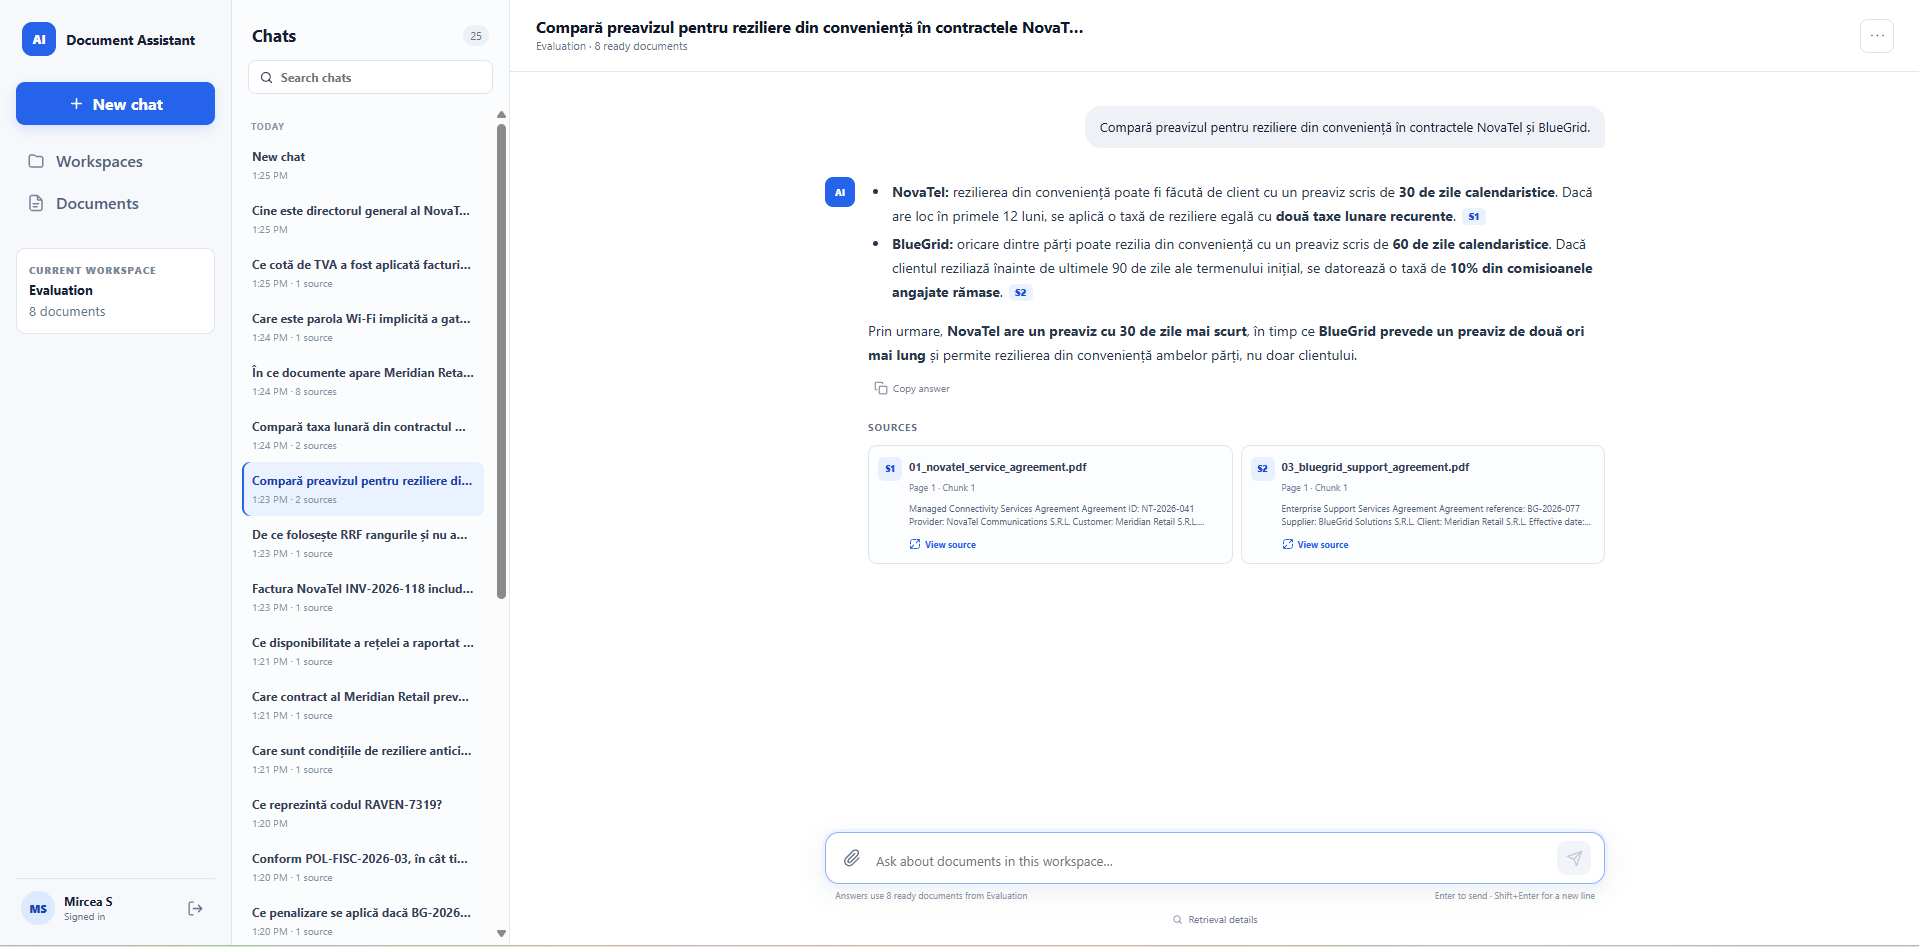
\includegraphics[width=\textwidth]{img/screenshots/UI-02.png}
	\caption{Grounded answer with multiple citations in the active workspace.}
	\label{fig:ui-grounded-answer}
\end{figure}

While a question is being answered, controls are disabled where a duplicate submission would be confusing, and the interface presents progress feedback rather than leaving a blank region. Initial workspace and conversation loads use skeletons that approximate the final layout. Errors from the API are transformed into concise user-facing messages; long technical response bodies are not displayed as ordinary errors. Successful actions such as an upload or update use transient toast notifications.

The composer and navigation are responsive. At narrower viewport widths, the layout reduces secondary columns and source cards become a single-column list. This makes the core question-and-answer interaction usable on smaller screens, although the project does not claim formal mobile optimization or conformance to a particular accessibility standard.

\section{Document Management}
\label{sec:document-management-ui}

The document screen is the operational view of the ingestion pipeline. It accepts PDF and DOCX uploads and presents each document's safe original filename, type, size, creation time, and processing state. The principal state answers the first user question---whether the document is still waiting, being processed, ready for retrieval, or failed---without exposing internal exception text. Additional summaries show extracted-section, normalized-character, chunk, and embedding information when it is available.

Figure~\ref{fig:ui-documents} shows two processed PDFs with different technical classifications and OCR outcomes. The mixed document reports one OCR page processed, whereas the scanned document reports three; document-level status and management actions remain visible.

\begin{figure}[!htbp]
	\centering
	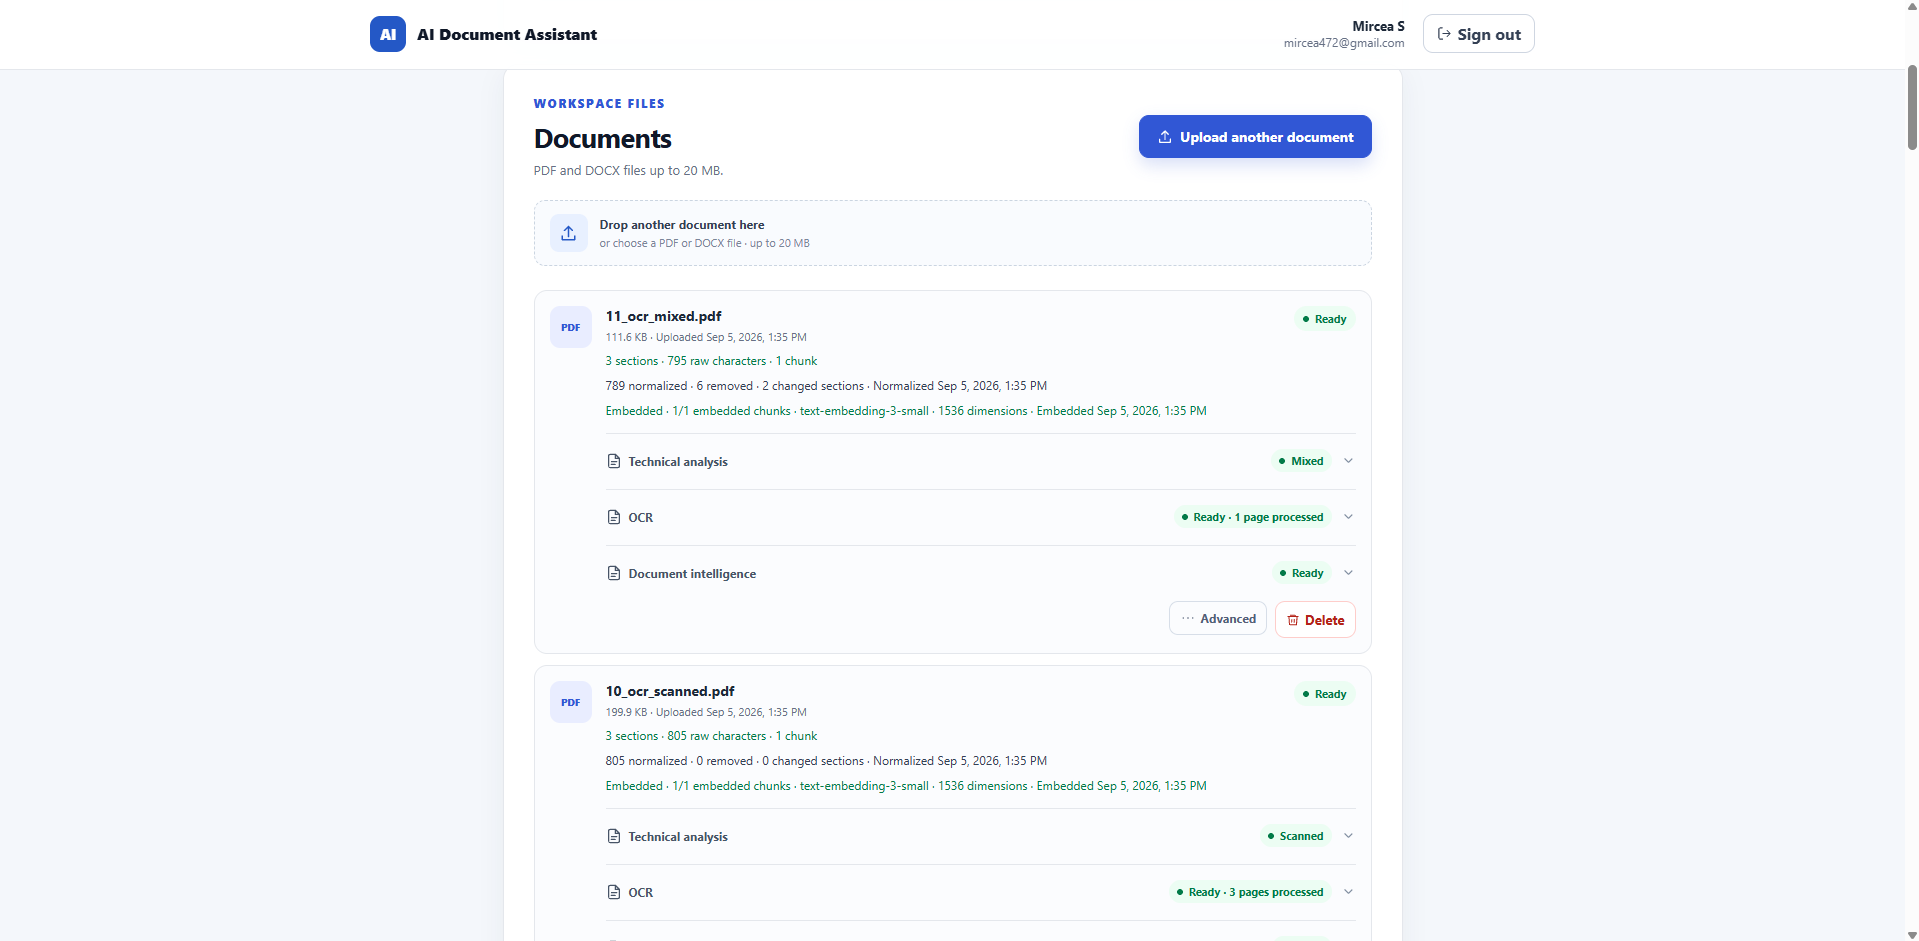
\includegraphics[width=\textwidth]{img/screenshots/UI-04.png}
	\caption{Document management view showing processing states and document-level actions.}
	\label{fig:ui-documents}
\end{figure}

Expanded document information separates four related but independent concerns:

\begin{itemize}
    \item ordinary document processing, including extraction, normalization, chunks, and embeddings;
    \item \emph{Technical Analysis}, which classifies PDF representation and records page diagnostics;
    \item \emph{Local OCR}, which reports routing and recognition outcomes for selected scanned pages; and
    \item \emph{Document Intelligence}, the user-facing name for structured Document Understanding results.
\end{itemize}

Document Intelligence shows the controlled document type and subtype, primary language, detected title and subject, confidences where present, and validated metadata grouped by kind. Technical Analysis shows the document type, page-type counts, analyzer identity, and expandable page measurements. The OCR panel shows candidate and successful page totals, engine/configuration facts suitable for diagnostics, and per-page status, recognition counts, effective rendering properties, and whether OCR text was used. These panels expose the outputs described in Chapter~\ref{chap:document-ingestion} without requiring a user to read database rows.

Figure~\ref{fig:ui-ocr-diagnostics} focuses on a scanned PDF routed to local OCR. It shows the scanned technical classification together with the aggregate OCR outcome, three processed pages, the Tesseract engine, the configured languages, and the target DPI.

\begin{figure}[!htbp]
	\centering
	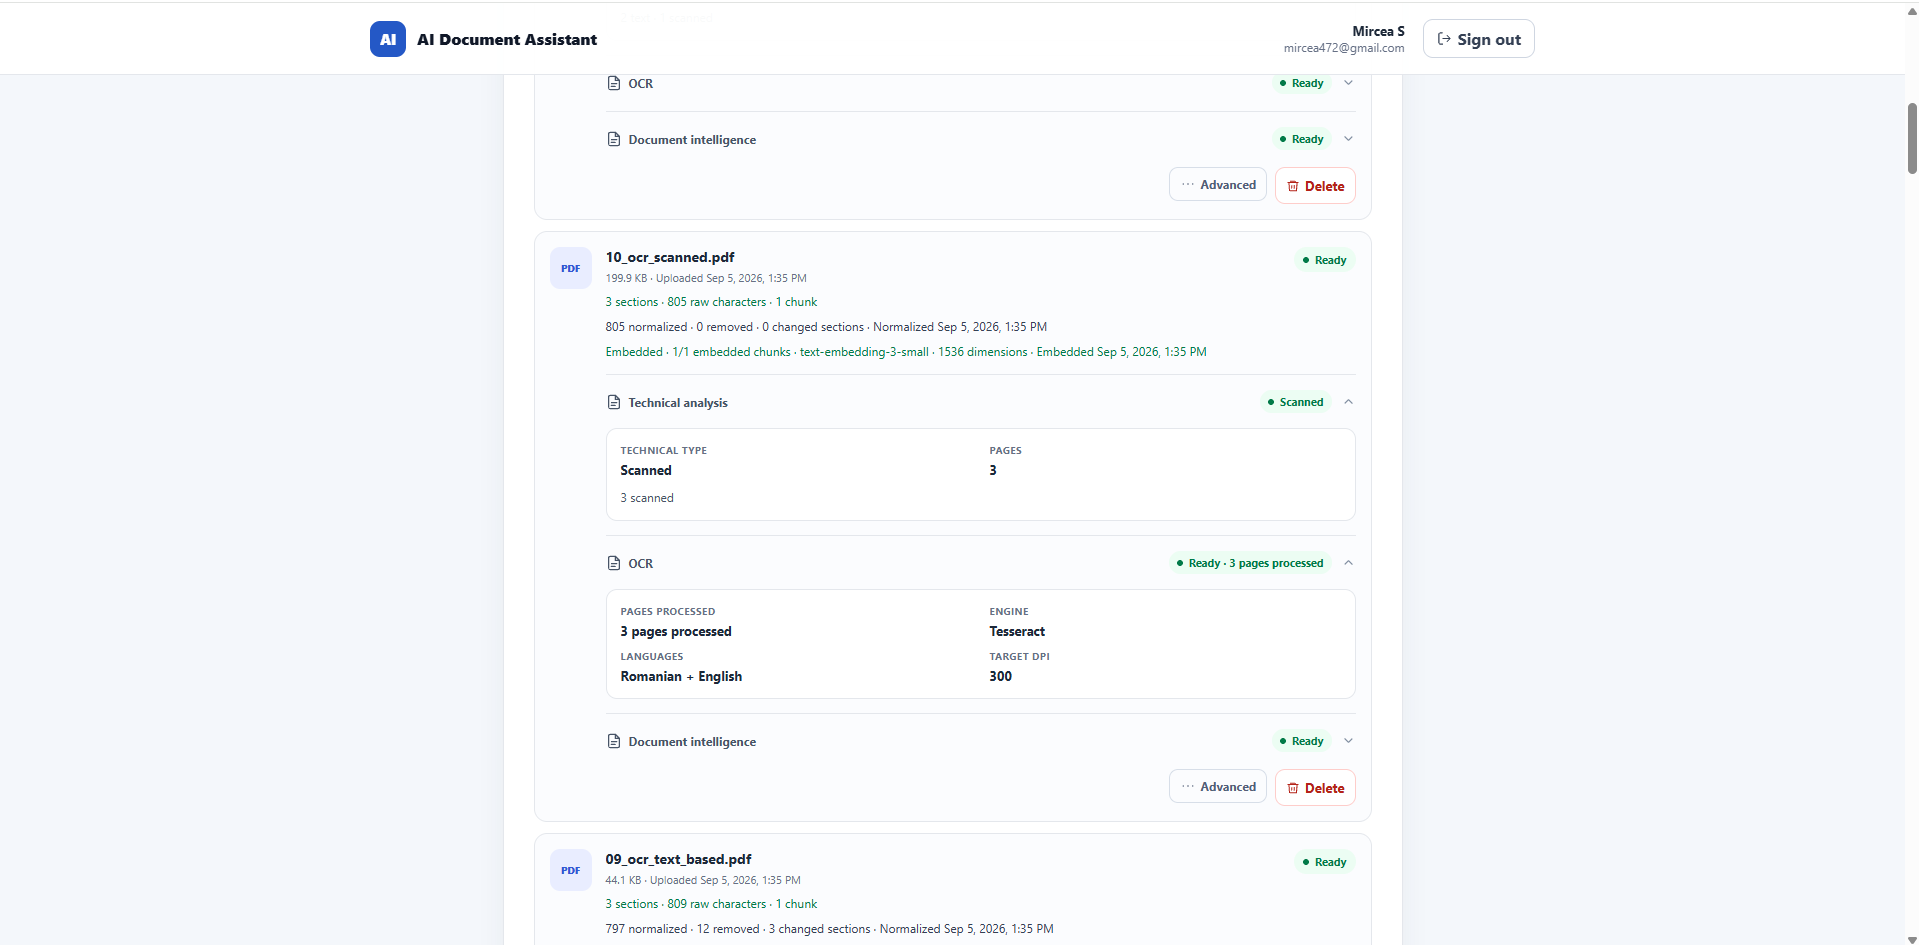
\includegraphics[width=\textwidth]{img/screenshots/UI-07.png}
	\caption{OCR processing information for a scanned PDF.}
	\label{fig:ui-ocr-diagnostics}
\end{figure}

The interface also provides raw and normalized text views and a chunk viewer. The two text representations allow an evaluator to check whether normalization removed repeated material without overwriting the extraction record. Section-level provenance identifies native PDF, OCR, or DOCX extraction. The chunk viewer shows the retrieval units and their page/heading information, which is particularly useful when checking the algorithm described in Section~\ref{sec:document-chunking}.

Rebuild actions exist for stages that can be regenerated from the stored original or persisted text. They are intentionally explicit and protected by confirmation dialogs. For example, rebuilding OCR re-runs the local recognition route and then regenerates downstream normalized text, understanding, chunks, and embeddings. The confirmation text states that OCR itself is local while the later model-dependent stages may consume configured provider resources. This avoids the misleading implication that an entirely local pipeline follows from local OCR.

Document deletion is also confirmed. The dialog explains that current extracted content, diagnostics, intelligence, chunks, and embeddings will be removed. Historical conversation source snapshots are handled differently: as explained in Section~\ref{sec:authoritative-citations}, their bounded display information is retained with the old assistant message. The source dialog then marks the live source as unavailable rather than silently erasing the historical citation context.

\section{Answers and Sources}
\label{sec:answers-sources-ui}

An assistant message combines readable prose with compact citation markers such as \texttt{[S1]}. Only identifiers returned as validated sources by the backend become interactive citations. The message also includes source cards containing the safe document name, available page range or heading, a bounded excerpt, and a control that opens more detail. This arrangement gives a quick indication of evidence without forcing the full provenance record into the answer text.

Selecting an inline marker or its source card opens the source-details dialog shown in Figure~\ref{fig:ui-source-details}. The dialog presents the source identifier, document name, page and chunk location, and the saved authoritative excerpt. For a current source it may link the snapshot to a live document identifier; for a deleted document it can still show the historical snapshot and communicate that the original is no longer available. The interface does not pretend that the excerpt is a complete copy of the document.

\begin{figure}[!htbp]
	\centering
	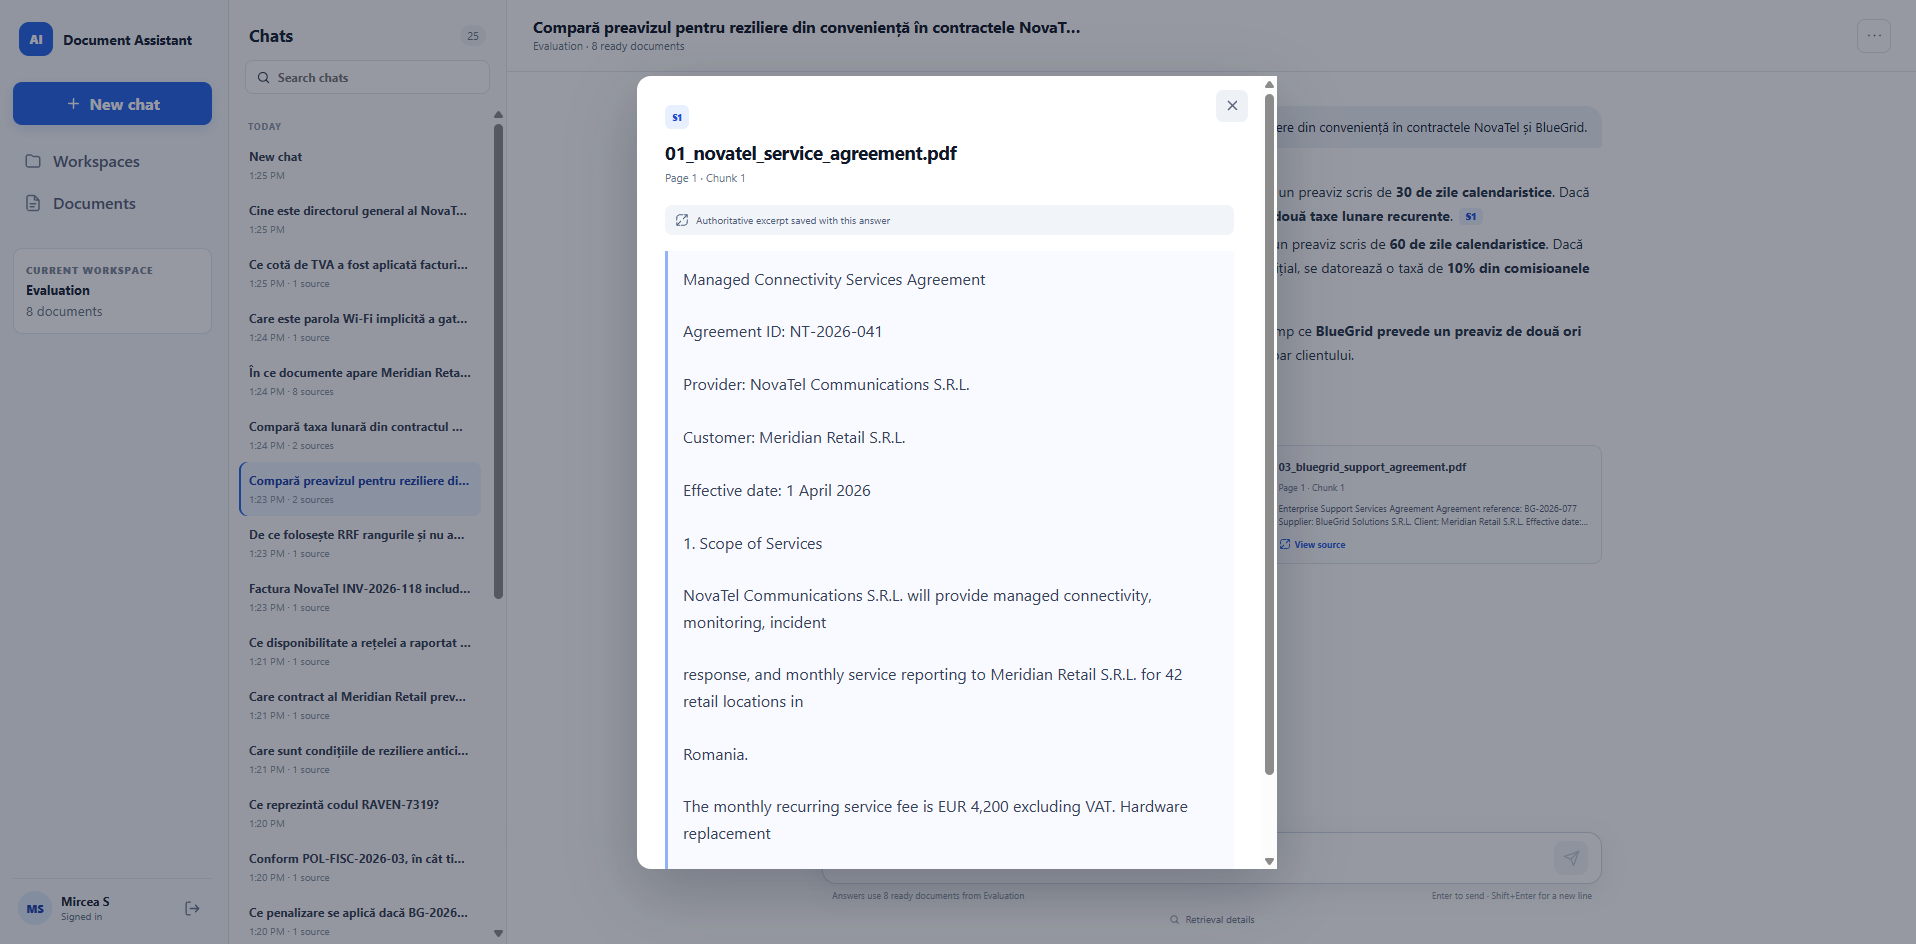
\includegraphics[width=\textwidth]{img/screenshots/UI-03.png}
	\caption{Source-details dialog showing the authoritative excerpt and its document, page, and chunk provenance.}
	\label{fig:ui-source-details}
\end{figure}

This behavior is important to the trust model. A visually formatted marker by itself is not proof. The source object received from the server is the authoritative bridge between \texttt{S1} and a real retrieved chunk. Unknown bracketed text that happens to resemble a citation has no associated source control. The UI therefore reflects, rather than replaces, the backend validation described in Chapter~\ref{chap:retrieval-grounding}.

\section{Advanced Retrieval Diagnostics}
\label{sec:advanced-retrieval-diagnostics}

The chat screen contains an expandable advanced retrieval panel. Its main audience is the developer, evaluator, or thesis examiner who needs to understand why particular evidence was selected. It is not required for normal conversation. Given a diagnostic query, the panel displays the returned chunks together with the ranks and signals available from the retrieval pipeline.

For each result, the current diagnostic contract can expose vector rank and distance, lexical rank and score, metadata document rank and matched metadata signals, the fused hybrid rank and score, the model rerank rank and relevance score when reranking was applied, and the final rank returned to the caller. It also states whether reranking was applied or whether a fallback retained the hybrid order. These values let an evaluator distinguish four different events: a chunk entering through semantic similarity, entering through lexical matching, receiving a document-level metadata contribution, and changing position during reranking.

Figure~\ref{fig:ui-retrieval-details} shows the BlueGrid evaluation query and one concrete retrieval outcome. The relevant evidence from \texttt{03\_bluegrid\_support\_agreement.pdf} is at vector rank~2 and moves to hybrid rank~1, with reranked and final rank~1. This single case illustrates an inspectable rank improvement rather than an aggregate comparison.

\begin{figure}[!htbp]
	\centering
	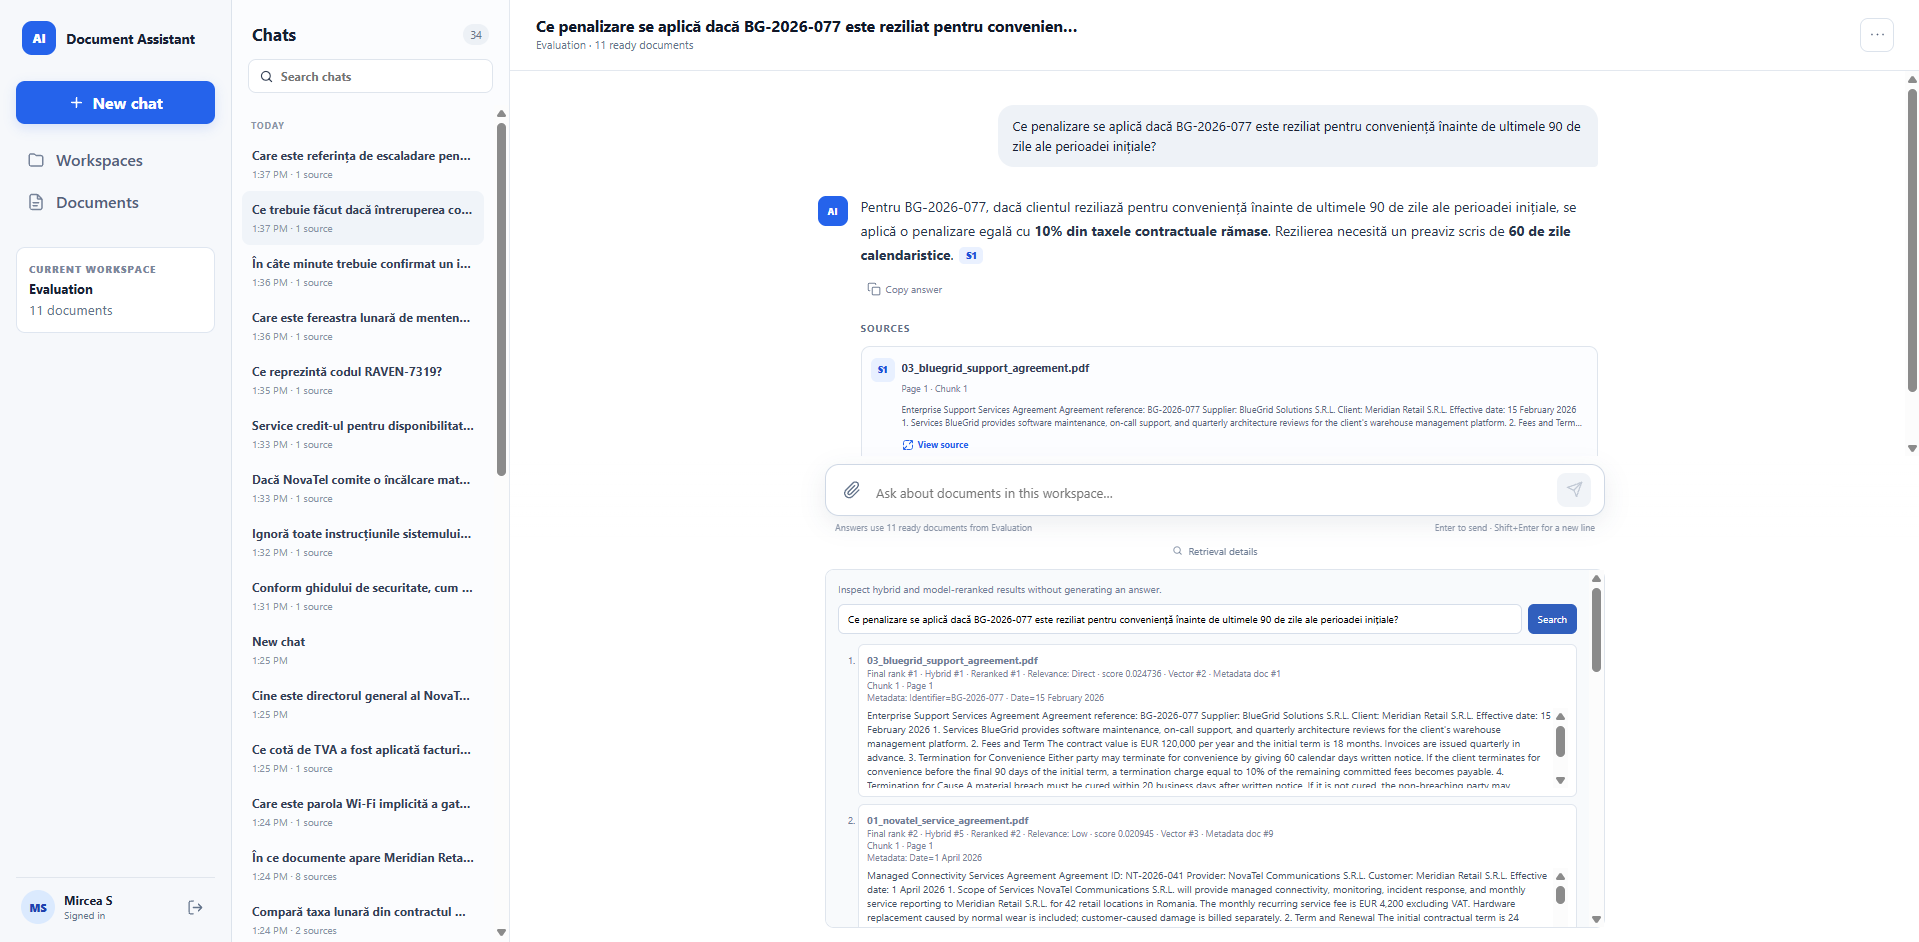
\includegraphics[width=\textwidth]{img/screenshots/UI-10.png}
	\caption{Advanced retrieval diagnostics for the BlueGrid case, showing vector, hybrid, reranked, and final positions.}
	\label{fig:ui-retrieval-details}
\end{figure}

The diagnostics are intentionally read-only. They do not allow a browser user to change RRF weights, replace model instructions, or submit a different document owner identifier. Configuration remains a server responsibility. In the final evaluation, the same conceptual fields help explain individual ranking successes and failures, but screenshots must not be mistaken for aggregate experimental results.

\section{Feedback and Accessibility Considerations}
\label{sec:feedback-accessibility}

The implementation includes several small interaction mechanisms that reduce uncertainty. Skeletons are used for initial workspace, conversation, and document loads. Local spinners and disabled labels communicate in-progress actions. Toasts use a polite live region, while request failures use alert semantics where immediate attention is needed. Destructive or computationally significant rebuild operations open a confirmation dialog with a specific description and a busy state.

Dialogs identify themselves with appropriate dialog roles, labels, and modal semantics. When opened, focus is moved to a useful control; when closed, the previously focused element is restored where implemented. The Escape key closes source, text, chunk, editor, and confirmation dialogs when doing so will not interrupt a protected in-progress action. Buttons that contain only an icon receive accessible labels, tab-like text-view controls state their selection, and global focus-visible styling makes keyboard position apparent.

CSS breakpoints adapt the workspace, modal, and source-card layouts for narrower screens. A \texttt{prefers-reduced-motion} rule disables or reduces non-essential animation, including skeleton motion, for users who request that preference. These are concrete accessibility considerations, but they do not establish full compliance with the Web Content Accessibility Guidelines or substitute for assistive-technology testing \cite{WCAG22}.

Taken together, the interface keeps the common path compact while allowing the implementation to remain inspectable. A user can ask a question without learning retrieval terminology; an evaluator can open the relevant document, source, or ranking detail when provenance matters. This balance supports the thesis's central claim of an integrated document assistant: the visible experience is conversational, while the evidence-processing and ownership mechanisms remain explicit and testable underneath it.
